% !TEX root = ../../../main.tex
%

\newpage
\section{Progettazione}
\subsection{Tipo di presa}

\begin{wrapfigure}{r}{5cm}
  \centering
  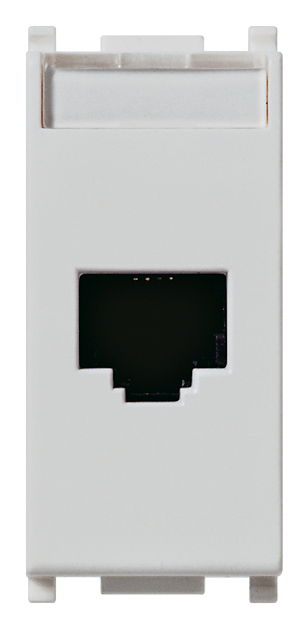
\includegraphics{vimar-14338-8-SL.jpg}
  \caption{Il connettore scelto per le prese utente.}\label{fig:presa}
\end{wrapfigure}

Supponendo che l'edificio abbia già alcune scatole elettriche incassate dedicate all'impianto di rete,
dove necessarie (anche condivise con altri connettori/controlli), non si terrà conto del costo di queste ultime.

Si sceglie di utilizzare prodotti di marca Vimar, serie Netsafe.
Nello specifico, si sceglie di usare dei connettori RJ45 Cat5e UTP (codice 14338.8.SL), illustrato in figura~\ref{fig:presa}.

Dato che determinate scatole elettriche possono contenere anche prese, pulsanti, interruttori o altri tipi
di dispositivi, non si conosce la dimensione (e di conseguenza il costo) delle placche decorative e dei supporti di montaggio.

Si suppone pertanto di affidarsi a quanto già predisposto per l'impianto elettrico (ove possibile).

Notare che nella maggior parte dei casi, questo non sarà necessario, in quanto gran parte dell'impianto,
per motivi di flessibilità e semplicità, verrà posato a pavimento, con delle prese direttamente disponibili sulle scrivanie.

Nei casi in cui è invece necessario affidarsi a delle prese a muro, resta valido quanto prima descritto.

\subsection{Dislocazione degli armadi e dorsale principale}

Data la topografia stellare del cablaggio orizzontale, si preferisce ospitare gli armadi per la \textit{floor distribution}
nei locali tecnici centrali all'edificio, in ogni piano. Essendo già stato fissato dalla planimetria fornita, il centralino
telefonico sarà per forza posizionato nel locale tecnico sud-ovest del piano terreno, assieme alle apparecchiature per
il collegamento alla rete pubblica.

Con questa scelta, il server (posizionato al piano terreno), godrà di una distanza ridotta con l'armadio di piano, garantendo
un miglior collegamento (in quanto si assume che il server necessiti di una considerevole quantità di banda), ed una maggiore
flessibilità nel caso in cui, in futuro, dovessero essere necessarie delle espansioni.

I collegamenti di dorsale dell'edificio saranno inizialmente orizzontali, dirette dal locale tecnico sud-ovest del piano terreno
verso quello centrale. Da quel punto, si muoveranno in verticale, raggiungendo gli altri armadi. La stessa cosa vale per i collegamenti
addizionali tra armadi adiacenti.

\subsection{Cablaggio orizzontale}

Si suppone di avere a disposizione un sistema di cablaggio a pavimento galleggiante, comprensivo di più canalette di larghezza sufficientemente
ampia da poter accogliere complessivamente, nelle parti iniziali del percorso, circa la metà di tutti i cavi utilizzati nel cablaggio di un singolo piano.

Per quanto concerne la sala riunioni, essendo adiacente al locale tecnico contenente l'armadio, ed essendo dotata di numerose prese,
si preferisce evitare di dover passare il cablaggio attraverso il corridoio: si preferisce attraversare il muro, predisposto con
un foro di diametro sufficiente, per raggiungere i tavoli da sotto il pavimento. Qui, le connessioni saranno poste al centro del tavolo principale
e su quello del presentatore mediante delle scatole elettriche oblique da scrivania.

Si ritiene utile sfruttare un passaggio simile per il raggiungimento della vicina sala server e, per i piani superiori,
del corridoio al lato opposto della porta presente nel locale tecnico. Non si ritiene ragionevole il percorrimento a ``U'' del corridoio
principale per il solo fine di raggiungere degli uffici altrimenti molto vicini in linea d'aria.

Queste considerazioni sono riportate nelle planimetrie che seguono (figure~\ref{fig:planimetria-terreno-cablaggio}~e~\ref{fig:planimetria-1-cablaggio}). I cablaggi di dorsale sono tracciati con delle linee
di spessore maggiore, ed i cerchi indicano il passaggio tra piani differenti.

Gli armadi sono evidenziati in azzurro e le prese in fuchsia.

Il cablaggio si distingue nel seguente modo:
\begin{description}
  \item[Verde] Fibra ottica multimodale 50/125.
  \item[Arancione] Cavi in rame Cat5e per Ethernet.
  \item[Rosso] Cavi in rame voice-grade (Cat3) per fonia.
\end{description}

\begin{figure}[ht]
  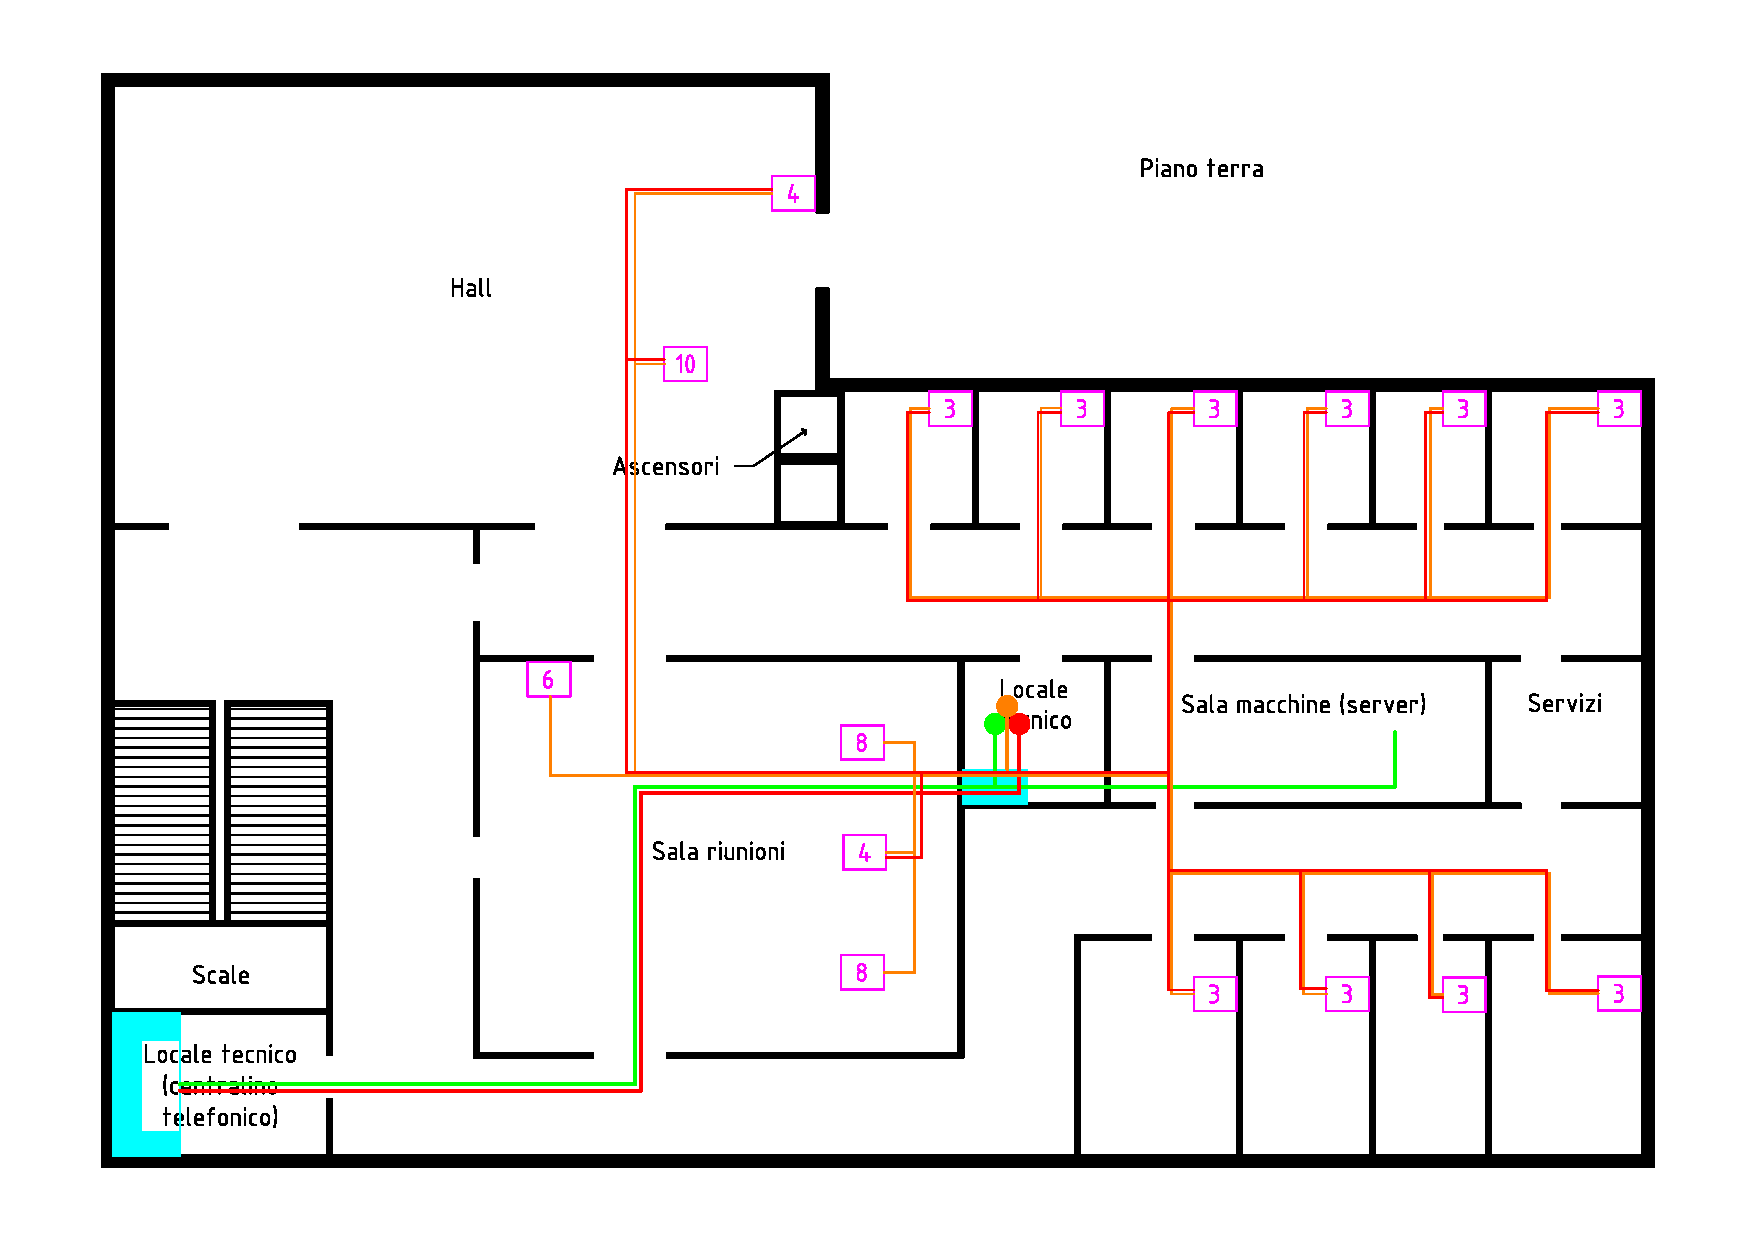
\includegraphics[angle=90,origin=c,width=\textwidth]{planimetrie-pianoterra-cablaggio}
  \caption{Cablaggio del piano terreno.}\label{fig:planimetria-terreno-cablaggio}
\end{figure}

\begin{figure}[ht]
  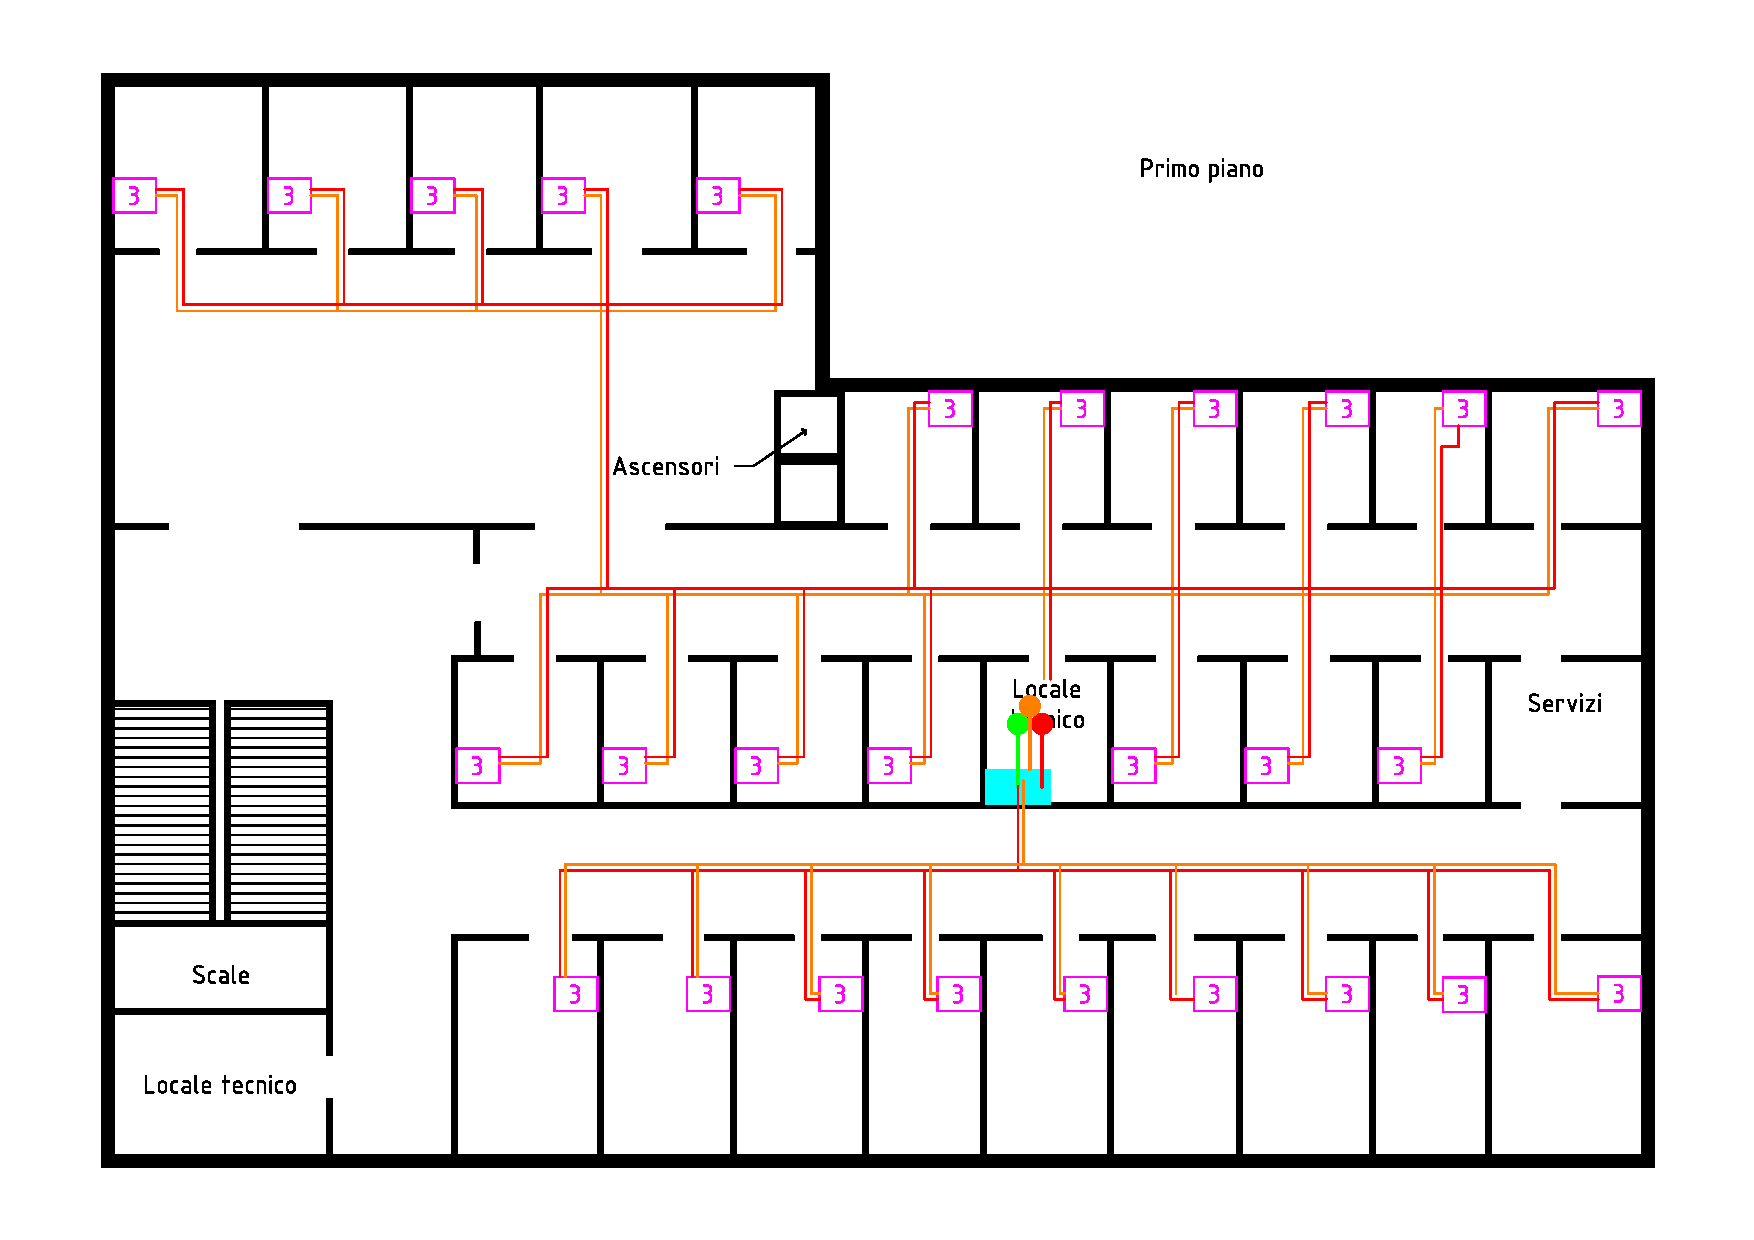
\includegraphics[angle=90,origin=c,width=\textwidth]{planimetrie-piano1-cablaggio}
  \caption{Cablaggio dei piani da primo a quarto.}\label{fig:planimetria-1-cablaggio}
\end{figure}

Si contano due pareti attraversate nel piano terra, e soltanto una per piano nei superiori.
